\documentclass[11pt]{article}
% fix quotes: https://tex.stackexchange.com/a/52353
\usepackage[english]{babel}
\usepackage{hyperref} % URLS
\usepackage{graphicx} % images
\usepackage{mathtools}
\usepackage{listings}
\usepackage{xcolor}
\usepackage{minted}
\usepackage{float}
 % no indent
\usepackage{parskip}
\usepackage[autostyle]{csquotes}
\usepackage{helvet}
% so we can stop latex hyphenating over new lines
%\usepackage[none]{hyphenat}
%\renewcommand{\familydefault}{\sfdefault}

% https://www.overleaf.com/learn/latex/Page_size_and_margins
\usepackage{geometry}
\geometry{
	a4paper,
	total={170mm,257mm},
	left=20mm,
	top=20mm,
}

% package instantiation
\MakeOuterQuote{"}
\hypersetup{
	colorlinks=true,
	linkcolor=blue,
	filecolor=magenta,
	urlcolor=cyan,
	citecolor=cyan,
}

% bibliography
% https://tex.stackexchange.com/questions/51434/biblatex-citation-order
% https://www.reddit.com/r/LaTeX/comments/k8tz0q/citation_in_wrong_numerical_order/
\usepackage[
    backend=biber,
    natbib=true,
    style=numeric,
    sorting=none
]{biblatex}
\addbibresource{major.bib}

% opening
\title{\textbf{A 3D music visualisation in OpenGL using the Discrete Fourier Transform}}
\author{Matt Young \\ 46972495 \\ m.young2@uqconnect.edu.au}
\date{May 2024}

\begin{document}
\maketitle

\begin{abstract}
    Constructing computer graphics from music has important implications in the field of live entertainment.
    The Discrete Fourier Transform (DFT), often computed via the Fast Fourier Transform (FFT), is the typical
    method to convert time domain audio signals to a frequency domain spectrum. With this spectral data comes
    an almost unlimited number of ways to interpret it and construct a visualisation. In this paper, I
    investigate applying the DFT to construct a semi real-time audio visualisation using OpenGL. The
    visualisation consists of offline spectral data that is rendered in real-time in the form of "bars" with
    lighting, and a set of pre-programmed camera moves computed via linear (translation) and
    spherical-linear (orientation) interpolation.
\end{abstract}

\tableofcontents

\clearpage
\listoffigures
\clearpage

\section{Introduction}
% Since the first music video in (YEAR) (CITE), there has been broad interest in constructing "music
% visualisers": the process of building an often real-time visual representation of the audio.

A \textit{music visualiser} is a computer program that takes as input an audio signal, typically music, and
produces as output a graphical visualisation. Technically, this can be an entirely offline process, but most
often music visualisers run in real-time. Music visualisers have an important role in the live entertainment
scene \cite{mccarthy2022live}, particularly for Electronic Dance Music (EDM). With an almost infinite number
of ways to interpret an audio signal, music visualisation is an eclectic mix of art and engineering.

\subsection{Visual inspiration}
The particular music visualiser I aim to construct is an improved version of the "spectrum of bars" once used
by Canadian record label Monstercat, shown in Figure \ref{fig:monstercat}.
The label has since transitioned away
from this computational music visualiser, and instead use custom music videos.

\begin{figure}[H]
\centering
\includegraphics[width=384px]{img/monstercat.png}
\caption{Visualisation of the song "Pure Sunlight" \cite{youtubeElectronicFijiWiji}}
\label{fig:monstercat}
\end{figure}

The visualisation in Figure \ref{fig:monstercat}
is a common type of visualisation that visualises the audio spectrum - it shows the magnitudes of the varying
frequencies that make up the song. This spectral data can be interpreted in a number of ways, for example, the
MilkDrop \cite{milkdrop} software includes visualisations that encode this in a number of complex ways. However,
for our use case, bars are visually appealing and an intuitive approach to visualising the music.

\section{Architecture overview}
\subsection{Overall description of sub-applications}
The visualiser itself is developed and tested in a Linux environment, and is split into two sub-applications:
the visualiser itself (written in C++20), and the analysis script (written in Python). Signal processing is a
very complex subject, and real-time ("online") signal processing in C++ is even more so. Python generally has
simpler tools to address signal processing problems, such as NumPy and SciPy, so the signal processing part
was moved offline into a Python script. This is shown in Figure \ref{fig:block}:

\begin{figure}[H]
\centering
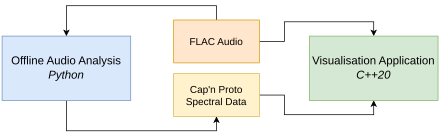
\includegraphics[width=300px]{img/diagram.drawio.png}
\caption{Block diagram of music visualisation application}
\label{fig:block}
\end{figure}

The analysis script is first run that reads a FLAC \cite{xiphFLACWhat} audio file, and produces a Cap'n Proto
\cite{capnp} encoded binary file containing the necessary data to render a spectrum for the chosen song. Each
song consists of a directory containing one audio file, \verb|audio.flac|, and one spectral data file,
\verb|spectrum.bin|. These are stored in the \verb|data| directory. For example: \\
\verb|data/songs/LauraBrehm_PureSunlight/{audio.flac},{spectrum.bin}|

Free Lossless Audio Codec (FLAC) \cite{xiphFLACWhat} is a lossless audio compression and container format. It was mainly selected
due to its ability to be easy loaded in C++ through open-source libraries like \verb|dr_flac|, the fact that
it's entirely royalty and patent free, as well as its lossless nature. Although codecs such as MPEG-3 and
Vorbis are transparent at around 320 Kbps (meaning there are no perceptible differences between the compressed
codec and uncompressed audio), there may still be subtle artefacts introduced in the spectrum that could be
picked up by the visualiser. In any case, storing the audio in an uncompressed format introduces very little
overhead and can always be transcoded later down the track if marginally smaller file size is desired.

Cap'n Proto \cite{capnp} is a binary serialisation format that is regarded as a faster successor to Protocol Buffers.
Compared to Protocol Buffers, which are also a widely used binary serialisation format, Cap'n Proto has the
added benefit of requiring zero decode time and supporting very fast in-memory access. This is perfect for the
spectral data, which needs to be written once by the Python code, and re-read continuously by the C++
rendering code. Some of this reading takes place in the audio callback, which could be regarded as a soft
real-time function, and hence requiring very minimal overhead.
\footnote{Additionally, Cap'n P integrates nicely with my editor, Neovim, which was one of the bigger reasons
for its selection.}

The FLAC file for a typical song weighs in at around 10 MB, and the spectral data is only around 200 KiB
thanks to Cap'n Proto's packed stream writing feature. Due to its speed, Cap'n P has to make some
trade-offs in regards to message size vs. speed, usually preferring larger messages. Since I'm checking the
data directory into the Git version control system, I used packed message writing to prefer smaller messages
with an ever so slightly longer decode time.

\subsection{Visualiser}
The visualiser is what we see on the screen, the real-time rendering system that displays the bars, once the
spectral data has been computed. It is written in C++20, uses the OpenGL graphics API, and is built using
industry standard tools CMake, Ninja and the Clang compiler. This code runs "online", meaning it runs in
real-time and we would ideally like to spend no longer than 16 ms per frame (for 60 FPS). It uses a number of
open-source libraries:
\begin{itemize}
	\item SDL2: Platform window management, keyboard/mouse inputs, OpenGL context creation
	\item glad: For OpenGL function loading and feature queries
    \item glm: The OpenGL maths library, used for computing transforms and its matrix/vector types
    \item Cap'n Proto: An extremely fast data serialisation format, used to transport data between Python and
        C++.
    \item dr\_flac: A fast single-file FLAC decoder.
    \item stb\_image: An image file decoder for many file formats.
\end{itemize}

\subsection{Analysis script}
The analysis script is written in Python, and computes the spectral data used by the visualiser to display the
bars. It computes this data "offline", meaning it does not run in real-time, unlike the C++ code. It also uses
a relatively standard setup of Python libraries, with some additions due to the audio work involved:
\begin{itemize}
    \item NumPy: Numerical computing library.
    \item SciPy: Scientific computing library.
    \item spectrum.py: Used to compute the periodogram.
    \item Cap'n Proto: Data inter-change format, see above.
    \item audiofile.py: For loading the FLAC file.
    \item Matplotlib: For graphing the waveform, debugging
\end{itemize}

\section{Signal processing}
The overarching goal of the signal processing is to turn a time-domain audio signal into a frequency domain
spectrogram, similar to the Monstercat visualiser shown in Figure \ref{fig:monstercat}.
This turns out to actually
be quite an involved process, so this section will essentially a whirlwind tour of audio signal processing!

\subsection{Background: Computer audio}
A raw audio signal consists of a number of digital \textit{samples} that are sent through
an audio system at a particular \textit{sampling frequency}, typically 44.1 KHz.
\footnote{The exact reasons why are out of scope for this paper, but it has to do with the Nyquist-Shannon
theorem and history with CDs.}
Most audio is stereo, and hence there are typically two channels (although cinemas, for example, may use many
more channels). Eventually making its way out of userspace and into the kernel, these samples are converted
into an analogue signal using a Digital-to-Analogue (DAC) converter, which is typically located on most PC
motherboards or as a separate peripheral. The samples cause the speaker \textit{driver} (the membrane, usually
driven by magnets) to vibrate, which creates the sensation of sound. A typical digital audio signal is shown
in Figure \ref{fig:audiosignal}.

In order to build the visualiser, we will need to convert this time-domain collection of samples into a
frequency-domain spectrogram.

\begin{figure}[H]
\centering
\includegraphics[width=350px]{img/audiosignal.png}
\caption{An audio signal loaded in Audacity. Top is zoomed out, bottom is zoomed in showing samples.}
\label{fig:audiosignal}
\end{figure}

\subsection{Fourier transforms, DFT and FFT}
The history of the Fourier transform dates back to 1822 when mathematician Joseph Fourier understood that any
function could be represented as a sum of sines \cite{wolframFourierSeries}. From that theory, the Fourier
transform was developed.

The core equation for the Fourier transform is given by \cite{wolframFourierTransform}:
$$\widehat{f}(\xi) = \int_{-\infty}^{\infty} f(x)\ e^{-i 2\pi \xi x}\,dx.$$

In simplistic terms, the Fourier transform converts a time-domain signal, where the $x$ axis is time and the
$y$ axis is magnitude, into the frequency-domain, where the $x$ axis is frequency and the $y$ axis is the
magnitude of that particular frequency. A diagram of this transform is shown in Figure \ref{fig:ftdiagram}.

\begin{figure}[H]
\centering
\includegraphics[width=250px]{img/fouriertransform.png}
\caption{Diagram showing the time-domain to frequency-domain conversion of the Fourier transform}
\label{fig:ftdiagram}
\end{figure}

From the Fourier transform comes the concept of the Discrete Fourier Transform (DFT). The equation for the DFT
is similar, but slightly different to, the equation for the regular continuous Fourier transform:
$$X_k = \sum_{n=0}^{N-1} x_n \cdot e^{-i2\pi \tfrac{k}{N}n}$$

The DFT itself has many applications outside of audio analysis. A close cousin of the DFT, the Discrete Cosine
Transform (DCT), is used in many image compression algorithms, for example.

Computing the DFT naively has a time complexity of $O(n^2)$ \cite{Rajaby2022} , which is typically considered
unfavourable in CS. This led to what has been described as "the most important numerical algorithm of our
lifetime" \cite{Strang1994}: the Fast Fourier Transform (FFT). The modern FFT was invented by James Cooley and
John Tukey in 1965 \cite{Cooley1965AnAF}, although Carl Freidrich Gauss had earlier work of a similar nature
from 1805 \cite{Heideman1985}. This algorithm reduces the complexity to $O(n \log n)$, which is much more
palatable.

It's also important to note here that evaluating the general DFT operates on complex numbers, and its result
is also complex. However, since we are using a real-valued audio signal, we can instead make use of
specialised variants of the FFT that use purely real signals \cite{Sorensen1987}. The complex output is then
just converted to its magnitude, e.g. given $z = x + yi$ we take $r = \sqrt{x^2 + y^2}$.

\subsection{Decoding and chunking audio}
In order for the Fourier transform to be possible, a \textit{chunk} of audio needs to be processed. In other
words, we can't just process individual samples since we're doing a time-domain to frequency-domain
transform. After decoding the FLAC audio using the \verb|audiofile| library, the audio samples are then split
into chunks/blocks of 1024 samples using NumPy. Additionally, the stereo signal is transformed into a mono
signal by averaging the left/right channels, since multi-channel FFTs are much more complicated.

This is all just a few lines of Python:
\begin{minted}{python}
    # load audio
    signal, sampling_rate = audiofile.read(song_path, always_2d=True)
    # assume a stereo signal, let's mix it down to mono
    mono = np.mean(signal, axis=0)
    # split signal into chunks of BLOCK_SIZE
    blocks = np.split(mono, range(BLOCK_SIZE, len(mono), BLOCK_SIZE))
\end{minted}

\subsection{Power spectrum and periodogram}
From the DFT, a power spectrum - otherwise known as "power spectral density" (PSD) - can be computed. The
power spectrum "describes how a signal's power is distributed in frequency" \cite{Youngworth2005}. Consider
a signal $U_T(t)$, whose Fourier transform is given by $|U_T(V)|^2$. The power spectrum can be computed as
follows, using the definition in \cite{Youngworth2005}:
$$\text{PS}(V) = \frac{|U_T(V)|^2}{N^2}$$
Where $N$ is the total number of sample points.

Then, the power spectral density can then be simply computed as:
$$\text{PSD}(V) = \frac{PS(V)}{\Delta v}$$
Where $\Delta v$ is the space between data points in frequency space (so, the sampling rate).

Critically, the result of this equation is in the units of amplitude squared per frequency unit - which is
unwieldy and not particularly useful for our type of audio analysis. Instead, it would be better if we
converted it into dBFS ("Decibels relative to full scale"). This is a unit where 0.0 dBFS is the loudest
possible sound a system can emit, and it decreases negatively from there. For example, -10 dBFS is 10 dB
quieter than the maximum possible sound a system can emit.

The conversion from PSD to dBFS can be achieved as follows, given our signal $U_T(t)$:

$$\text{dbFS}_T(t) = \sum_t \log_{10} \frac{\text{PSD}(t)}{\text{max(PSD)}}$$

Implementing the above in Python, this produces the plot in Figure \ref{fig:psd}:

\begin{figure}[H]
\centering
\includegraphics[width=385px]{img/psd.png}
\caption{Power spectral density (PSD) in dbFS of a block of audio from the song "Saturn's Air" by
    artist Animadrop.}
\label{fig:psd}
\end{figure}

Also to note here is that we compute a metric known as \textit{spectral energy}, which is a measure of the
"excitement" of the audio. It's computed as the magnitude squared of the FFT:
$$S_E = \sum_{i=0}^{k} (\text{PSD}(i))^2$$

\subsection{Binning spectral data}
Now that we have spectral data for each block of audio, we need to process it into "bins", or blocks, and use
that to construct the bars. Given we know the number of bars we want (by default, 32), we can simply sample
this using NumPy:

\begin{minted}{python}
    samples = np.linspace(FREQ_MIN, FREQ_MAX, NUM_BARS)
\end{minted}

Where \verb|FREQ_MIN| and \verb|FREQ_MAX| refer to the human hearing range, 20 Hz to 20 KHz, respectively.

Then, we simply walk through the linear space considering our current and previous value, and compute the mean
amplitude inside this block. There is some additional code that maps this value, in dbFS, to a \verb|uint8_t|
bar height from 0 to 255, for Cap'n Proto serialisation.

Once this is computed, the data is serialised and can be loaded in C++ - and the signal processing is
complete.

\section{Computer graphics}
\subsection{Audio and spectrum decoding}

\subsection{Transforming and rendering bars}

\subsection{Computing camera animations}
In the visualiser, camera animations really consist of a begin pose, end pose, and a duration. This is
encoded in the \verb|cosc::CameraAnimation| class. Then, in turn, a
\verb|cosc::CameraAnimationManager| is attached to the \verb|cosc::Camera|, which enables it to animate the
camera every frame.

\begin{minted}[fontsize=\footnotesize]{c++}
/// A camera animation
class CameraAnimation {
public:
    /// Beginning camera pose
    CameraPose begin;
    /// Ending camera pose
    CameraPose end;
    // Duration of the animation in seconds
    float duration;

    explicit CameraAnimation(const CameraPose &poseBegin, const CameraPose &poseEnd, float time) :
        begin(poseBegin), end(poseEnd), duration(time) {};
};

/// Manages a camera with a set of animations.
class CameraAnimationManager {
public:
    explicit CameraAnimationManager(Camera &camera) : camera(camera) {};

    void update(float delta);

    void addAnimations(std::vector<CameraAnimation> animation) {
        ...
    }

    ...
};
\end{minted}

The \verb|cosc::CameraPose| represents both the position and orientation of the camera using a 3D vector and
quaternion respectively. TODO explain quaternions (lol).

\section{Results}

\section{Discussion}
Future improvements, etc.

\section{Self-assessment}

\section{Conclusion}

\section{References}
\printbibliography[heading=none]

\end{document}
